\documentclass[12pt,pdf,hyperref={unicode}]{beamer}
%\usetheme{boxes}
\beamertemplatenavigationsymbolsempty
\setbeamertemplate{footline}[page number]
% Set it for the internal PhD thesis defence to reduce number of slides
%\setbeamersize{text margin left=0.5em, text margin right=0.5em}

\usepackage[utf8]{inputenc}
%\usepackage[english, russian]{babel}
\usepackage{bm}
\usepackage{multirow}
\usepackage{ragged2e}
\usepackage{indentfirst}
\usepackage{multicol}
\usepackage{subfig}
\usepackage{amsmath,amssymb}
\usepackage{enumerate}
\usepackage{mathtools}
\usepackage{comment}
\usepackage[all]{xy}
\usepackage{tikz}
\usetikzlibrary{positioning,arrows}
\tikzstyle{name} = [parameters]
\definecolor{name}{rgb}{0.5,0.5,0.5}

%\usepackage{caption}
%\captionsetup{skip=0pt,belowskip=0pt}

%\newtheorem{theorem}{Theorem}
%\newtheorem{statement}{Statement}
%\newtheorem{definition}{Definition}

% colors
\definecolor{darkgreen}{rgb}{0.0, 0.2, 0.13}
\definecolor{darkcyan}{rgb}{0.0, 0.55, 0.55}
%\AtBeginEnvironment{figure}{\setcounter{subfigure}{0}}
%\captionsetup[subfloat]{labelformat=empty}

%----------------------------------------------------------------------------------------------------------

\title{Struggling with popularity bias in recommendation systems}
%\author{Name Surname}
%\institute[]{}
%\date{2024}

%---------------------------------------------------------------------------------------------------------
\begin{document}
%\begin{frame}
%\titlepage
%\end{frame}
\setcounter{page}{2}%remove here for the title
%----------------------------------------------------------------------------------------------------------
%\section{Please do not use sectioning in the presentations}
\begin{frame}{Struggling with popularity bias in RS}
\begin{block}{Long-tail problem}
In RS a small fraction of popular items account for the majority of user interactions. When trained on such data, the model usually gives higher scores to popular items than their ideal values while simply predicting unpopular items as negative.
\end{block}
\begin{block}{Agent-Based Modeling}
provides a playground for simulation of user interactions on synthetic data and measure the bias without running AB on real users.
\end{block}
\begin{block}{The solution} Using the agent-based model we provide a guide how to setting classical methods of struggling with popularity bias without running AB on real users.
\end{block}
\end{frame}
%----------------------------------------------------------------------------------------------------------
\begin{frame}{Long-tails in real data}
The plots show the interaction counts for each item within the dataset on the x-axis, sorted in descending order. 
\begin{columns}
\begin{column}{0.3\textwidth}
The Gini index expresses the inequality of the distribution, with values closer to 1 indicating a high inequality (range: 0–1)
\end{column}
\begin{column}{0.7\textwidth}
	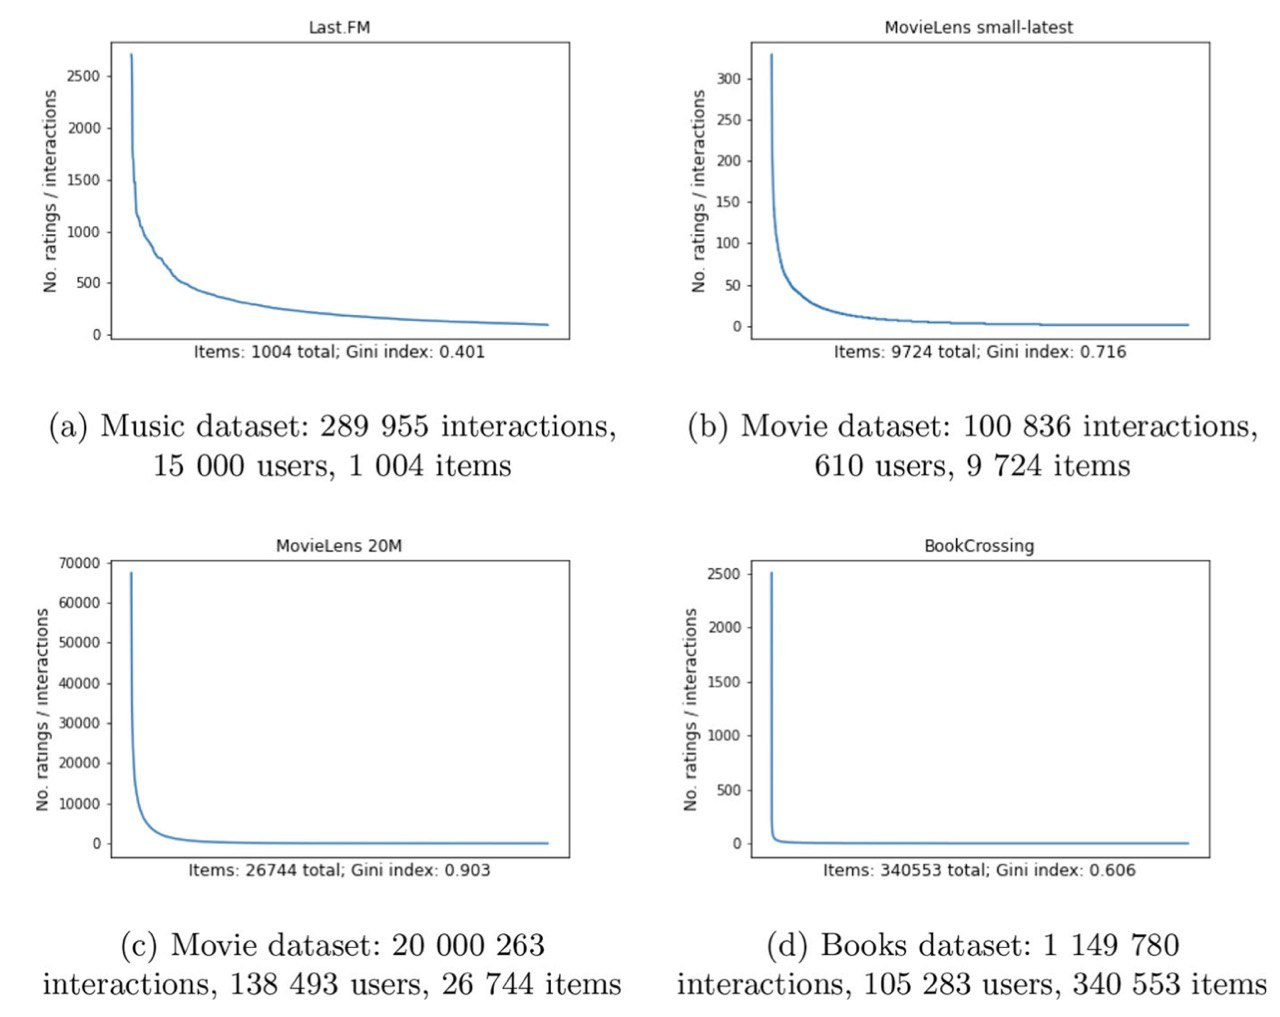
\includegraphics[width=1\textwidth]{Step 1/long_tails_plots.jpg}      
\end{column}
\end{columns}
\bigskip
Popularity bias exists in almost all of the popular datasets.
\end{frame}
\end{document}